\documentclass{article}

\usepackage{extramarks}

\usepackage{amsmath}
\usepackage{amsthm}
\usepackage{amssymb}
\usepackage{amsfonts}
\usepackage{caption}
\usepackage{subcaption}
\usepackage{listings}

\usepackage{hyperref}

\usepackage{tikz}

\usepackage{algorithm}
\usepackage{algorithmic}
\usepackage[shortlabels]{enumitem}

\usepackage{float,graphicx}

\usepackage{pgfplots}

\usepackage{adjustbox}


\usepackage{array}
\usepackage{pgfgantt}

\usepackage[utf8]{inputenc}

\usepackage{fancyhdr}
\usepackage{fancybox}

\topmargin=-0.45in
\evensidemargin=0in
\oddsidemargin=0in
\textwidth=6.5in
\textheight=9.0in
\headsep=0.25in

% Listings' Styles

\definecolor{codegreen}{rgb}{0,0.6,0}
\definecolor{codegray}{rgb}{0.5,0.5,0.5}
\definecolor{codepurple}{rgb}{0.58,0,0.82}
\definecolor{backcolour}{rgb}{0.96,0.96,0.96}


\lstdefinestyle{python}{
    backgroundcolor=\color{backcolour},
    commentstyle=\color{codegreen},
    keywordstyle=\color{magenta},
    numberstyle=\tiny\color{codegray},
    stringstyle=\color{codepurple},
    basicstyle=\footnotesize,
    breakatwhitespace=false,
    breaklines=true,
    captionpos=b,
    keepspaces=true,
    numbers=left,
    numbersep=5pt,
    showspaces=false,
    showstringspaces=false,
    showtabs=false,
    tabsize=2
}

\lstset{style=python}
\lstset{language=Python}

\linespread{1.1}
\captionsetup[table]{position=bottom}

\pagestyle{fancy}
\lhead{\groupName}
\chead{\hmwkClass: \hmwkTitle}
\rhead{\today}
\lfoot{\lastxmark}
\cfoot{\thepage}

\renewcommand\headrulewidth{0.4pt}
\renewcommand\footrulewidth{0.4pt}
\renewcommand\qedsymbol{$\blacksquare$}

\setlength\parindent{0pt}

\newcommand{\hmwkTitle}{Assignment Sheet\ \#\hmwkNumber}
\newcommand{\hmwkDueDate}{April 5, 2022}
\newcommand{\hmwkClass}{Machine Learning}
\newcommand{\hmwkAuthorName}{Henri Sota, Enis Mustafaj}
\newcommand{\groupName}{\textbf{Group HB}}

% Homework Number Variable
\newcommand{\hmwkNumber}{8}

%
% Create Problem Sections
%

\newcommand{\enterProblemHeader}[1]{
    \nobreak{}
}

\newcommand{\exitProblemHeader}[1]{
    \stepcounter{#1}
}

\setcounter{secnumdepth}{0}
\newcounter{partCounter}
\newcounter{homeworkProblemCounter}

\setcounter{homeworkProblemCounter}{1}
\nobreak\extramarks{Problem \hmwkNumber \arabic{homeworkProblemCounter}}{}\nobreak{}

%
% Homework Problem Environment
%
% This environment takes an optional argument. When given, it will adjust the
% problem counter. This is useful for when the problems given for your
% assignment aren't sequential. See the last 3 problems of this template for an
% example.
%
\newenvironment{homeworkProblem}[1][-1]{
    \ifnum#1>0
        \setcounter{homeworkProblemCounter}{\hmwkNumber.#1}
    \fi
    \section{Problem \hmwkNumber.\arabic{homeworkProblemCounter}}
    \setcounter{partCounter}{1}
    \enterProblemHeader{homeworkProblemCounter}
}{
    \exitProblemHeader{homeworkProblemCounter}
}


\newcounter{programmingPartCounter}
\newcounter{programmingProblemCounter}

\setcounter{programmingProblemCounter}{1}
\nobreak\extramarks{Programming Problem \hmwkNumber \arabic{programmingProblemCounter}}{}\nobreak{}

%
% Programming Problem Environment
%
% This environment takes an optional argument. When given, it will adjust the
% problem counter. This is useful for when the problems given for your
% assignment aren't sequential. See the last 3 problems of this template for an
% example.
%
\newenvironment{programmingProblem}[1][-1]{
    \ifnum#1>0
        \setcounter{programmingProblemCounter}{\hmwkNumber.#1}
    \fi
    \section{Programming Problem \hmwkNumber.\arabic{programmingProblemCounter}}
    \setcounter{programmingPartCounter}{1}
    \enterProblemHeader{programmingProblemCounter}
}{
    \exitProblemHeader{programmingProblemCounter}
}

\title{
    \vspace{2in}
    \textmd{\textbf{\hmwkClass:\\ \hmwkTitle}}\\
    \normalsize\vspace{0.1in}\small{Due\ on\ \hmwkDueDate\ at 10:00}\\
    \vspace{3in}
}

\author{\groupName \\ \hmwkAuthorName}
\date{}

\renewcommand{\part}[1]{\textbf{\large Part \Alph{partCounter}}\stepcounter{partCounter}\\}

% Useful for algorithms
\newcommand{\alg}[1]{\textsc{\bfseries \footnotesize #1}}

% Alias for the Solution section header
\newcommand{\solution}{\textbf{\large Solution}}
\newcommand{\comment}[1]{} % Multi-line comment

\DeclareMathOperator*{\argmax}{arg\,max}
\DeclareMathOperator*{\argmin}{arg\,min}

\begin{document}
\maketitle
\pagebreak
\begin{homeworkProblem}
In this exercise, we repeat the general idea of the bias-variance trade-off for growing model complexity. To this end, you are asked to provide one plot that gives curves for the irreducible error, the bias, the variance, and the total (expected) generalization error for growing model complexity. \textit{(You might have seen such a plot in the lecture material.)} In addition, comment in your own words the "behavior" of the four different curves. Again, in your own words, explain, in connection to these curves, the idea of the bias-variance trade-off.

\begin{center}
    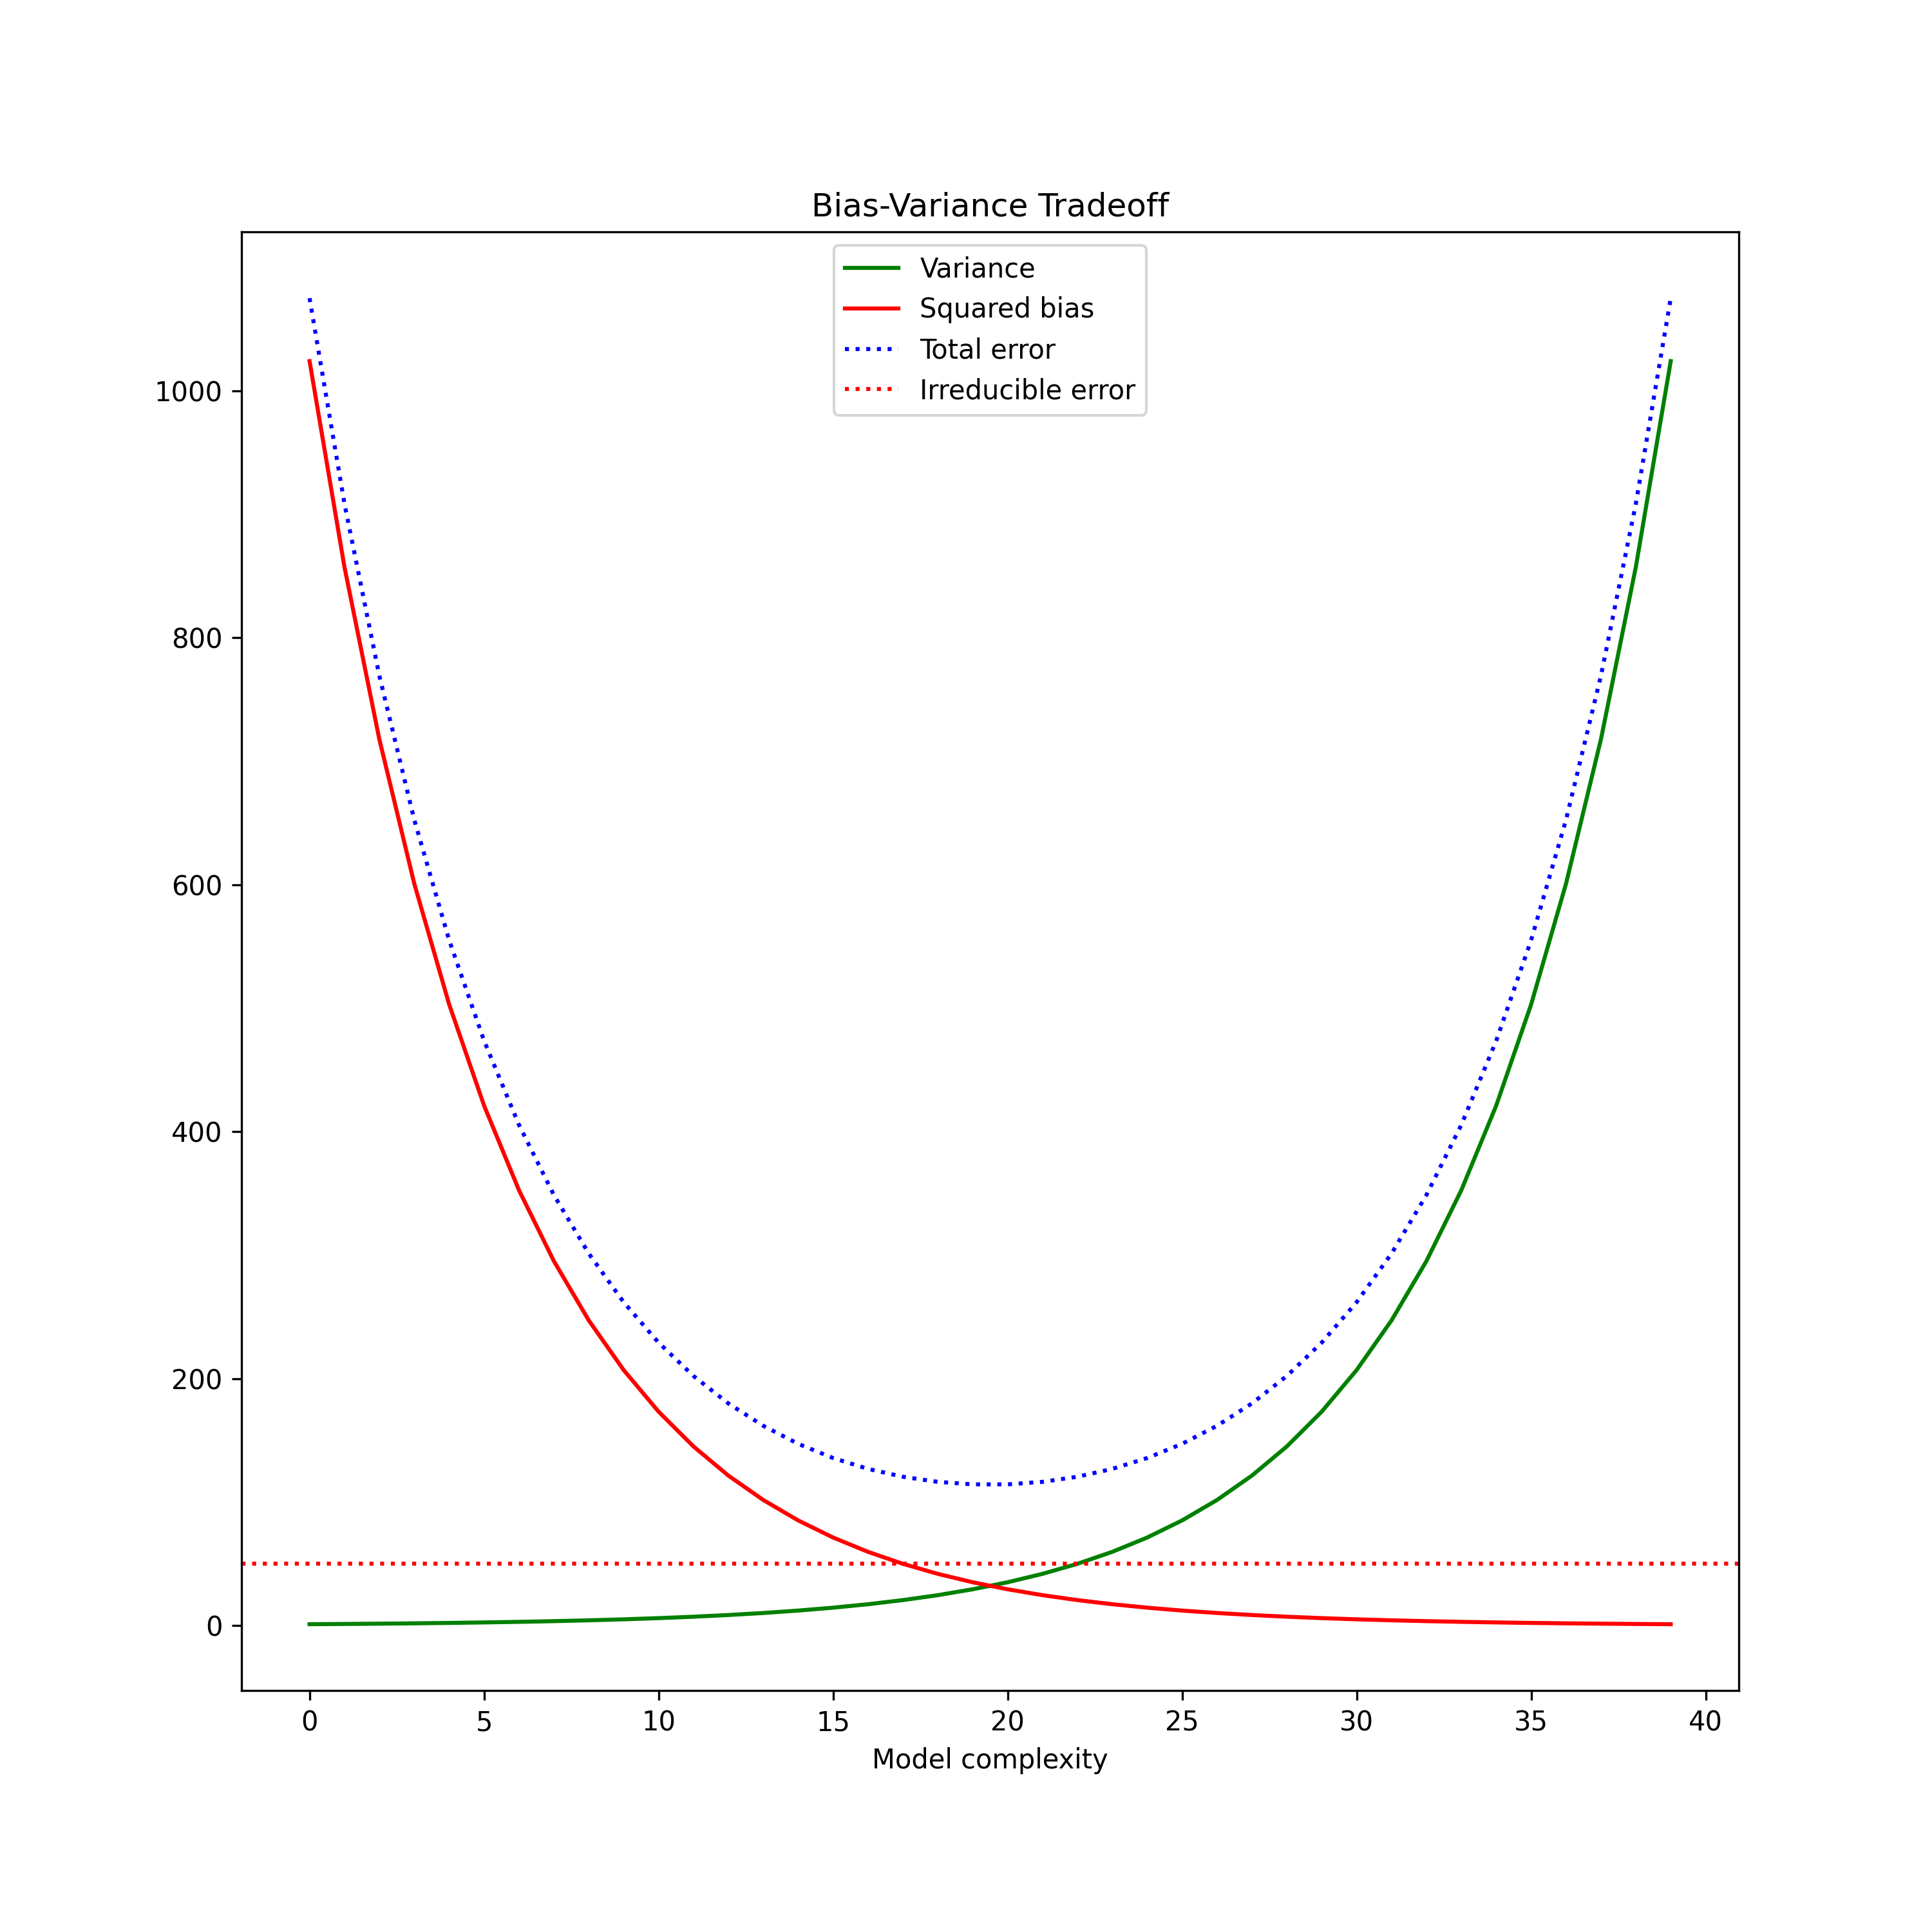
\includegraphics[width=0.6\textwidth]{bias_variance_plot.png}
\end{center}

In the plot above, we can see the relationship between (squared) bias, variance, irreducible error and total (expected) generalization error.
\begin{itemize}
    \item The irreducible error is constant, independent of the model complexity, due to random noise. It is inherent to the collected data. The irreducible error can represent noise coming from collection of data, from the non-deterministic behavior of the phenomenon being modelled, and generally, any type of noise that cannot be easily defined.
    \item The bias error arises from erroneous assumptions in the learning algorithm of the model. It represents the difference between the average of the predicted value over different realizations of training data and the true value. A model with high bias oversimplifies the underlying model from which the data has been generated from and it misses to predict complex and relevant relations between the input and output. This is known as \textit{underfitting}. The bias error curve typically has a high value for low model complexity and low value for high model complexity. This arises from the fact that with increased model complexity, the model is able to make more assumptions about the data and to capture the complex relations in the data.
    \item The variance error arises from sensitivity to small fluctuations in the training set. It represents the mean squared deviation of the predicted value from its expected value over different realizations of training data. A model with high variance fits to the training data quite well, but it suffers in other cases due to its inability to generalize beyond the training data. This is known as \textit{overfitting}. The variance curve typically has a low value for low model complexity and high value for high model complexity. This arises from the fact that with increased model complexity, the model starts to fit the training data too well with the aim to minimize the training error. As a result, the model will show different performance with similar datasets.
    \item The total (expected) generalization error is the sum of the irreducible error, the bias error and the variance error. Therefore its behavior depends on the behavior of the other curves.
\end{itemize}

The bias-variance trade-off is based on the choice of increasing or decreasing the model complexity to lower bias (increase variance) or lower variance (increase bias) with the aim to reduce the total (expected) generalization error. The model should accurately capture the underlying model in its training data while generalizing well to data that it has not seen before. It is typically impossible to do both simultaneously. Models with high bias produce simpler models that may underfit the data. On the other side, models with high-variance may overfit the data and perform poorly in different scenarios. Therefore, the trade-off lies in adjusting the model used with the aim to reduce both errors theoretically.
\end{homeworkProblem}
\pagebreak
\begin{homeworkProblem}
Recall from the lecture that the general bias-variance decomposition is given by
\begin{equation*}
    EGE(f, \textbf{x}_{0}) = \sigma_{\varepsilon}^{2} + \left [ \text{E}_{T}[f_{T}(\textbf{x}_{0}) \right ] - f_{exact}(\textbf{x}_{0})]^{2} + \text{E}_{T} \left [ (f_{T}(\textbf{x}_{0}) - \text{E}_{T}[f_{T}(\textbf{x}_{0})])^{2} \right ]
\end{equation*}

While in the lecture notes, we discuss this decomposition more concretely for kNN regression, we do not discuss it for linear regression by least squares. Since deriving the resulting decomposition for linear regression by least squares is a bit involved, we will not do this here. Instead, we want to compute the bias and variance term for concretely given data and the linear model trained via the least squares estimator.

To achieve this, we first assume to have $f_{exact}(x) = x^{2}$. Moreover, we consider the four samples $\mathcal{T}_{1} = \{ x_{i}^{(1)}, y_{i}^{(1)} \}_{i = 1}^{3}$, $\mathcal{T}_{2} = \{ x_{i}^{(2)}, y_{i}^{(2)} \}_{i = 1}^{3}$, $\mathcal{T}_{3} = \{ x_{i}^{(3)}, y_{i}^{(3)} \}_{i = 1}^{3}$, $\mathcal{T}_{4} = \{ x_{i}^{(4)}, y_{i}^{(4)} \}_{i = 1}^{3}$ from $T$ with $N = 3$ training samples. These are given as follows
\begin{table}[H]
    \centering
    \begin{tabular}{|c|c|c|c|c|}
        \hline
        $t$ & $i$ & $x_{i}^{(t)}$ & $\varepsilon_{i}^{(t)}$ & $y_{i}^{(t)} = f_{
        exact}(x_{i}^{(t)}) + \varepsilon_{i}^{(t)}$ \\ \hline \hline
        1 & 1 & -1.0 & -0.3 & \\
        1 & 2 & -1.5 & 0.2 & \\
        1 & 3 & 0.5 & 0.1 & \\ \hline
        2 & 1 & -0.5 & 0.0 & \\
        2 & 2 & 1.5 & -0.2 & \\
        2 & 3 & -1.5 & 0.3 & \\ \hline
        3 & 1 & 1.5 & -0.1 & \\
        3 & 2 & 2.0 & 0.0 & \\
        3 & 3 & -0.5 & 0.1 & \\ \hline
        4 & 1 & 1.0 & -0.2 & \\
        4 & 2 & -2.0 & 0.1 & \\
        4 & 3 & 1.5 & 0.3 & \\ \hline
    \end{tabular}
\end{table}

Finally we choose $x_{0} = 0$.
\begin{enumerate}[a)]
    \item Compute the output samples of the given training sets, i.e. fill in the remaining cells in the above table.
    
    After the calculations, the output samples will be:
    
    \begin{table}[H]
        \centering
        \begin{tabular}{|c|c|c|c|c|}
            \hline
            $t$ & $i$ & $x_{i}^{(t)}$ & $\varepsilon_{i}^{(t)}$ & $y_{i}^{(t)} = f_{
            exact}(x_{i}^{(t)}) + \varepsilon_{i}^{(t)}$ \\ \hline \hline
            1 & 1 & -1.0 & -0.3 & 0.7 \\
            1 & 2 & -1.5 & 0.2 & 2.45\\
            1 & 3 & 0.5 & 0.1 & 0.35\\ \hline
            2 & 1 & -0.5 & 0.0 & 0.25\\
            2 & 2 & 1.5 & -0.2 & 2.05\\
            2 & 3 & -1.5 & 0.3 & 2.55\\ \hline
            3 & 1 & 1.5 & -0.1 & 2.15\\
            3 & 2 & 2.0 & 0.0 & 4\\
            3 & 3 & -0.5 & 0.1 & 0.35\\ \hline
            4 & 1 & 1.0 & -0.2 & 0.8\\
            4 & 2 & -2.0 & 0.1 & 4.1\\
            4 & 3 & 1.5 & 0.3 & 2.55\\ \hline
        \end{tabular}
    \end{table}
    
    \pagebreak
    
    
    \item Now that you have all four training sets at hand, compute an estimator for the bias term. To this end, you first build for all four different training sets the linear model using linear regression by least squares, hence you obtain models $f_{\mathcal{T}_{1}}, f_{\mathcal{T}_{2}}, f_{\mathcal{T}_{3}}, f_{\mathcal{T}_{4}}$. You then need to estimate the expectation, recalling that for a random variable $Z$ an estimator for its mean is given by
    \begin{equation*}
        \text{E}(Z) \approx \bar{Z} = \frac{1}{M} \sum_{i = 1}^{M} z_{i}
    \end{equation*}

    where the $z_{1}, \ldots, z_{M}$ are $M$ samples drawn from that random variable. \textit{Hint: Use a computer to find the necessary partial results.}
    
    The final training sets are:
    \begin{equation*}
        \mathcal{T}_{1} = \{(-1, 0.7), (-1.5, 2.45), (0.5, 0.35)\}
    \end{equation*}
    \begin{equation*}
        \mathcal{T}_{2} = \{(-0.5, 0.25), (1.5, 2.05), (-1.5, 2.55)\}
    \end{equation*}
    \begin{equation*}
        \mathcal{T}_{3} = \{(1.5, 2.15), (2, 4), (-0.5, 0.35)\}
    \end{equation*}
    \begin{equation*}
        \mathcal{T}_{4} = \{(1, 0.8), (-2, 4.1), (1.5, 2.55)\}
    \end{equation*}
    
    By using the least squares formula:
    \begin{equation*}
        \beta = (\mathcal{X}^{T} \cdot \mathcal{X})^{-1} \cdot \mathcal{X} \cdot y
    \end{equation*}
    
    we calculate the coefficients vector of the model for each training set:
    \begin{itemize}
        \item $\mathcal{T}_{1}$:
            \begin{equation*}
                \beta = \Bigg(\begin{pmatrix} 1 & 1 & 1 \\ -1 & -1.5 & 0.5 \end{pmatrix} \cdot 
                \begin{pmatrix}1 & -1 \\ 1 & -1.5 \\ 1 & 0.5 \end{pmatrix}\Bigg)^{-1} \cdot \begin{pmatrix} 1 & 1 & 1 \\ -1 & -1.5 & 0.5 \end{pmatrix} \cdot \begin{pmatrix}0.7 \\ 2.45 \\ 0.35 \end{pmatrix}
            \end{equation*}
            \begin{equation*}
                \beta =  \begin{pmatrix}0.59230769 \\ -0.86153846\end{pmatrix}
            \end{equation*}
            The predictor for $\mathcal{T}_{1}$ is $f_{\mathcal{T}_{1}}(x) = 0.59230769 -0.86153846 \cdot x $ and the predicted value at $x_{0}$ is $f_{\mathcal{T}_{1}}(x_{0}) = 0.5923076923076922$
            
        \item $\mathcal{T}_{2}$:
            \begin{equation*}
                \beta = \Bigg(\begin{pmatrix} 1 & 1 & 1 \\ -0.5 & 1.5 & -1.5 \end{pmatrix} \cdot 
                \begin{pmatrix}1 & -0.5 \\ 1 & 1.5 \\ 1 & -1.5 \end{pmatrix}\Bigg)^{-1} \cdot \begin{pmatrix} 1 & 1 & 1 \\ -0.5 & 1.5 & -1.5 \end{pmatrix} \cdot \begin{pmatrix}0.25 \\ 2.05 \\ 2.55 \end{pmatrix}
            \end{equation*}
            \begin{equation*}
                \beta =  \begin{pmatrix}1.61428571 \\ -0.01428571\end{pmatrix}
            \end{equation*}
            The predictor for $\mathcal{T}_{2}$ is $f_{\mathcal{T}_{2}}(x) = 1.61428571 -0.01428571 \cdot x $ and the predicted value at $x_{0}$ is $f_{\mathcal{T}_{2}}(x_{0}) = 1.6142857142857139$
            
        \item $\mathcal{T}_{3}$:
            \begin{equation*}
                \beta = \Bigg(\begin{pmatrix} 1 & 1 & 1 \\ 1.5 & 2 & -0.5 \end{pmatrix} \cdot 
                \begin{pmatrix}1 & 1.5 \\ 1 & 2 \\ 1 & -0.5 \end{pmatrix}\Bigg)^{-1} \cdot \begin{pmatrix} 1 & 1 & 1 \\ 1.5 & 2 & -0.5 \end{pmatrix} \cdot \begin{pmatrix}2.15 \\  4 \\ 0.35\end{pmatrix}
            \end{equation*}
            \begin{equation*}
                \beta =  \begin{pmatrix}0.86666667 \\ 1.3\end{pmatrix}
            \end{equation*}
            The predictor for $\mathcal{T}_{3}$ is $f_{\mathcal{T}_{3}}(x) = 0.86666667 + 1.3 \cdot x $ and the predicted value at $x_{0}$ is $f_{\mathcal{T}_{3}}(x_{0}) = 0.8666666666666669$
            
        \item $\mathcal{T}_{4}$:
            \begin{equation*}
                \beta = \Bigg(\begin{pmatrix} 1 & 1 & 1 \\ 1 & -2 & 1.5 \end{pmatrix} \cdot 
                \begin{pmatrix}1 & 1 \\ 1 & -2 \\ 1 & 1.5 \end{pmatrix}\Bigg)^{-1} \cdot \begin{pmatrix} 1 & 1 & 1 \\ 1 & -2 & 1.5 \end{pmatrix} \cdot \begin{pmatrix}0.8 \\ 4.1 \\ 2.55 \end{pmatrix}
            \end{equation*}
            \begin{equation*}
                \beta =  \begin{pmatrix}2.59534884 \\ -0.67209302\end{pmatrix}
            \end{equation*}
            The predictor for $\mathcal{T}_{4}$ is $f_{\mathcal{T}_{4}}(x) = 2.59534884 -0.67209302 \cdot x $ and the predicted value at $x_{0}$ is $f_{\mathcal{T}_{4}}(x_{0}) = 2.595348837209302$
    \end{itemize}
    
    By using the formula above, we calculate the expected value of $f_{T}(0)$:
    \begin{equation*}
        E_{T}[f_{T}(0)] \approx \frac{1}{4} \cdot \sum_{i=1}^{4}f_{\mathcal{T}_{i}}(0) = 1.4171522276173438
    \end{equation*}
    
    Now we can calculate the bias:
    
    \begin{equation*}
        bias =  \text{E}_{T}[f_{T}(\textbf{x}_{0})] - f_{exact}(\textbf{x}_{0}) = 1.4171522276173438
    \end{equation*}
    \item Finally estimate the variance term. Here, it is useful to further observe that the variance term is indeed the variance of $f_{T}(\textbf{x}_{0})$ with respect to the random variable $T$, hence
    \begin{equation*}
        \text{E}_{T} \left [ (f_{T}(\textbf{x}_{0}) - \text{E}_{T}[f_{T}(\textbf{x}_{0})])^{2} \right ] = \text{Var}_{T}(f_{T}(\textbf{x}_{0}))
    \end{equation*}
    
    Then use that an unbiased estimator for the variance of a random variable $Z$ is given by
    \begin{equation*}
        \text{Var}(Z) \approx \frac{1}{M - 1} \sum_{i = 1}^{M} (z_{i} - \bar{Z})^{2}
    \end{equation*}
    
    \textit{Hint: Use a computer to find the necessary partial results.}
    
    By using the formula above, we calculate the variance:
    \begin{equation*}
        \text{Var}_{T}(f_{T}(\textbf{x}_{0})) \approx \frac{1}{3} \cdot \sum_{i=1}^{4}(f_{\mathcal{T}_{i}}(0) - E_{T}[f_{T}(0)]) = 0.8034705742217966
    \end{equation*}
\end{enumerate}
\end{homeworkProblem}
\begin{programmingProblem}
In this programming exercise, we further study Example 7.2 from the lecture notes with its associated implementation. If we more carefully read the example, we observe that in the process of the evaluation of the different error contributions, we build $N_{T} = 100$ different kNN regression predictors for $k = 1, \ldots, 20$. Note however, that these predictors are only built from the training data $\{ (x_{i}, f_{exact}(x_{i}) \}_{i = 1}^{N}$ and not from $\{ (x_{i}, f_{exact}(x_{i}) + \varepsilon_{i}) \}_{i = 1}^{N}$.
\begin{enumerate}[a)]
    \item Start by extending the existing implementation such that you also build all these predictors for the training data with the additional noise term.
    
    The implementation has been extended and can be found in the file \texttt{programming\_exercises.ipynb}.
    \item Now, fix $k = 3$ and add a plot that contains the evaluation of all these predictors (with included noise term). Thus you obtain a total of $N_{T} = 100$ different curves. Try to use some appropriate coloring and transparency to make them properly visible.\\
    The plot that you will then have created is a visualization of the variance of the predictor.
    
    \begin{center}
    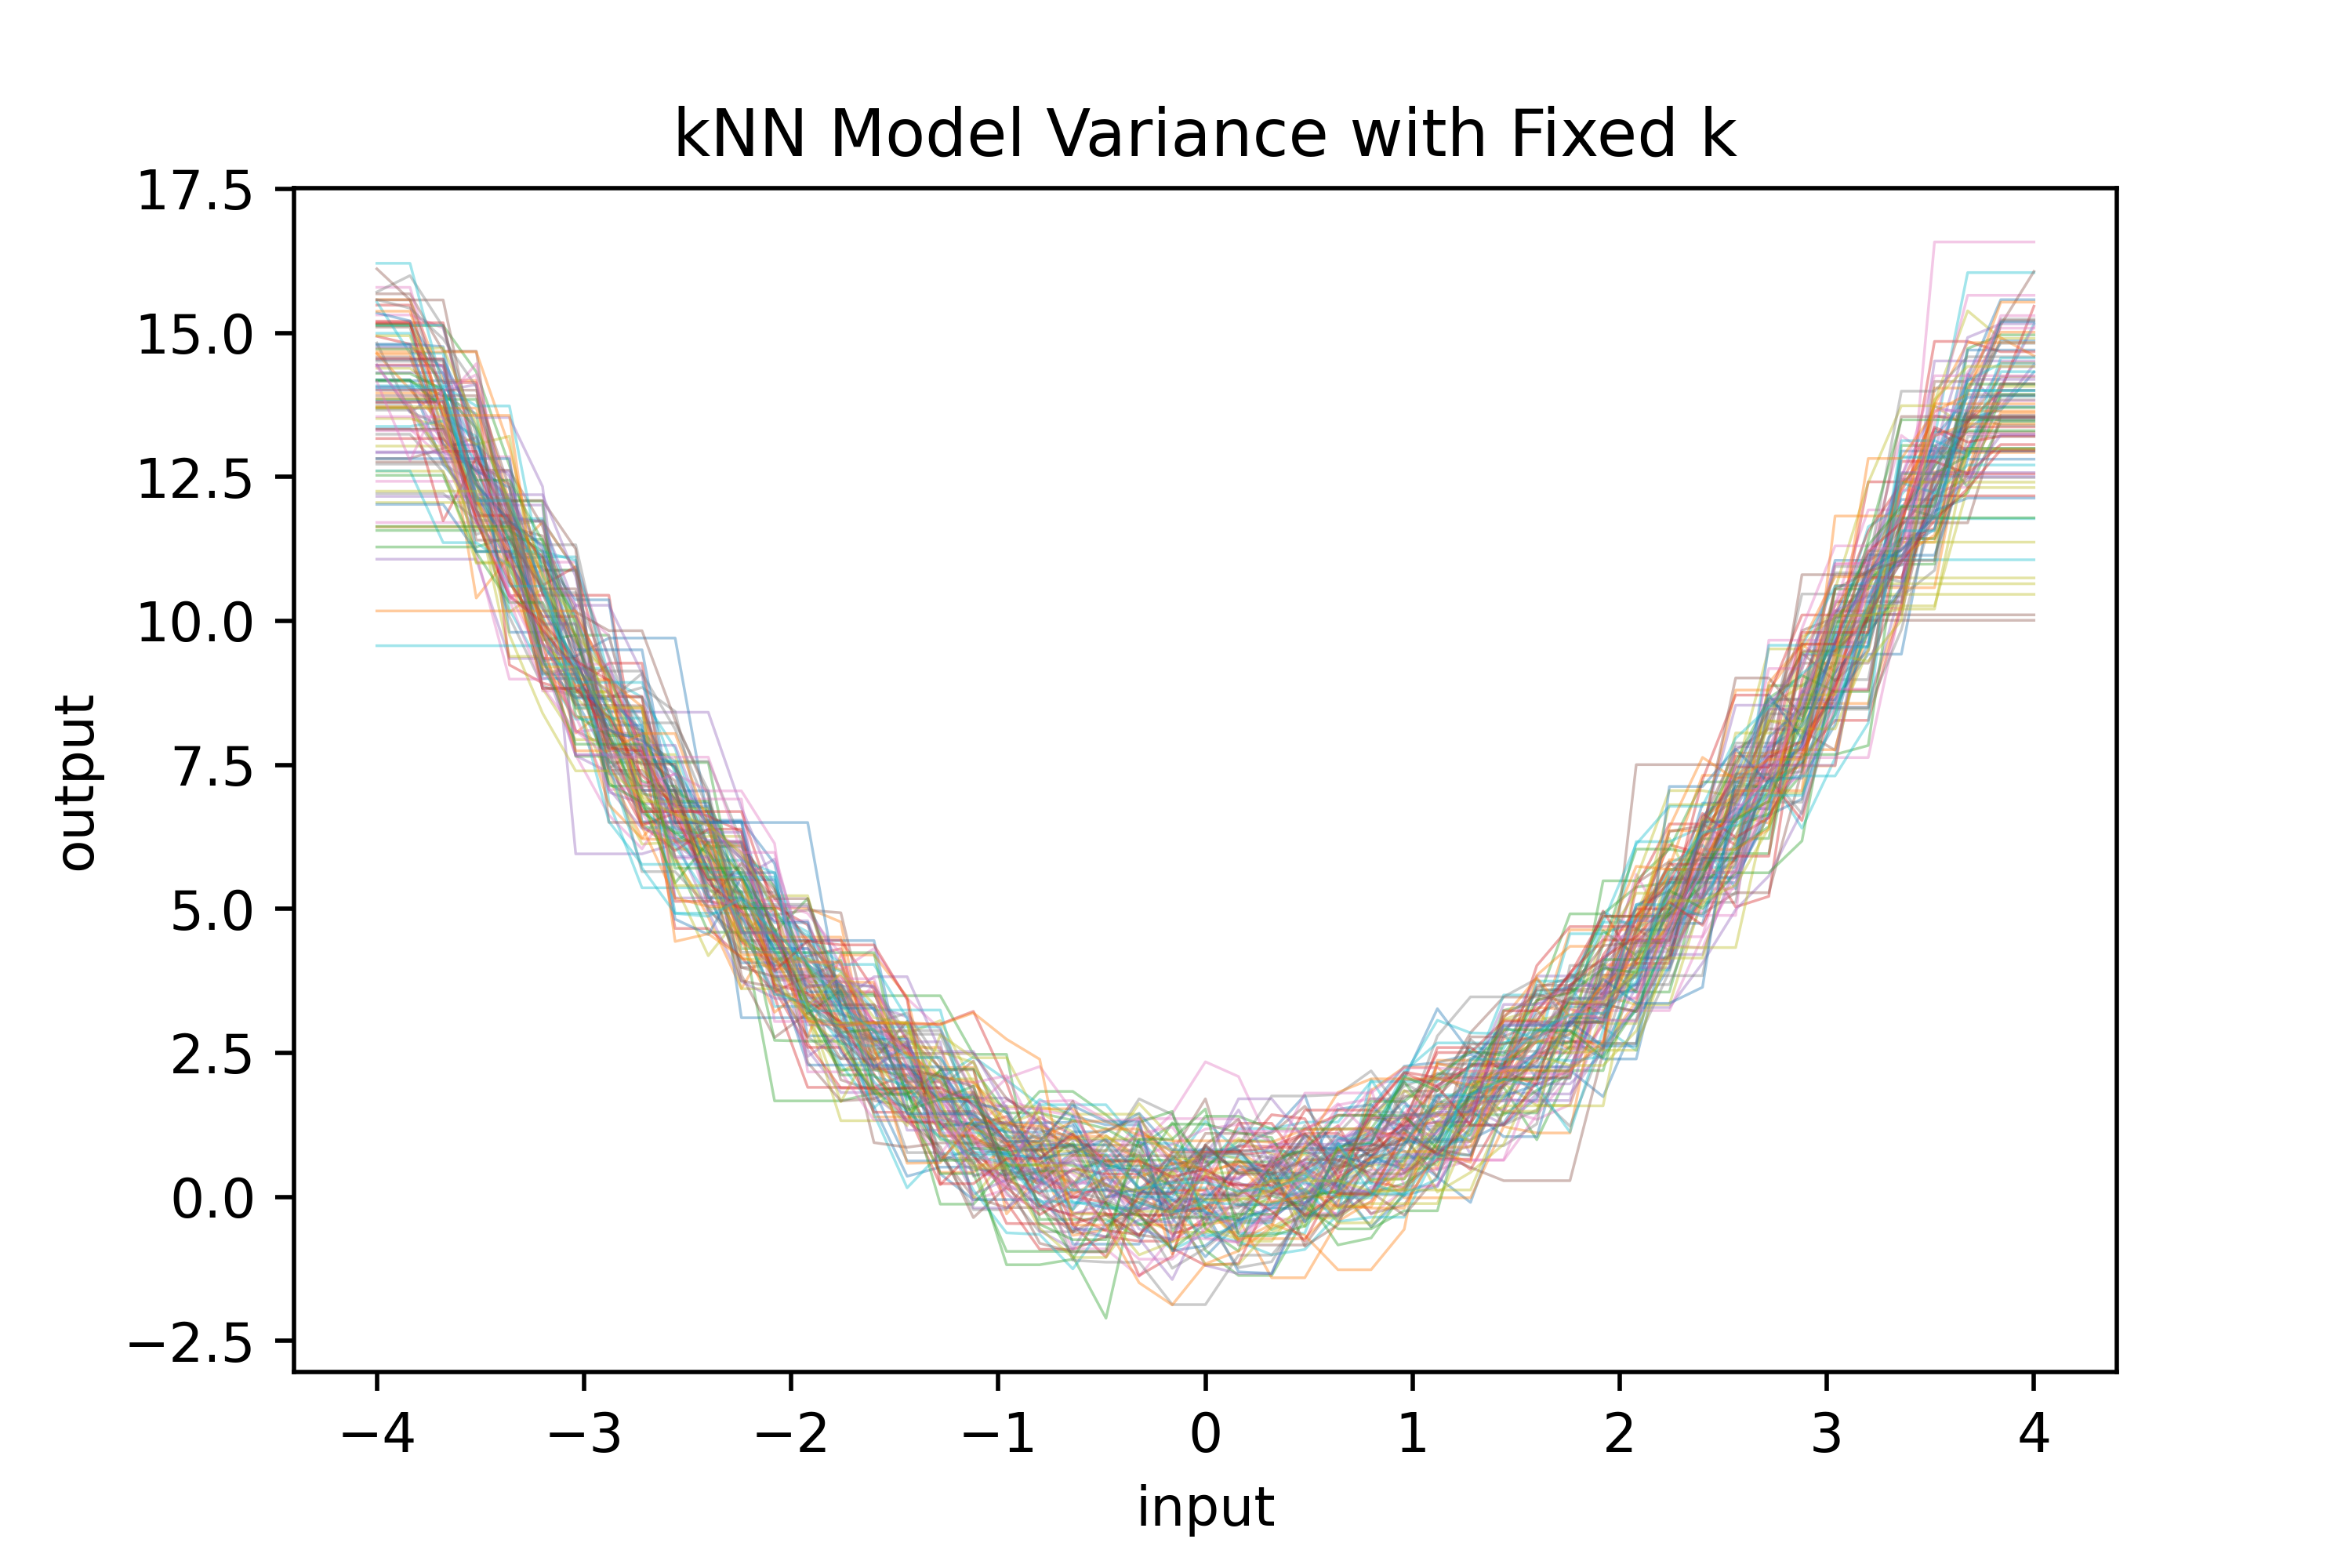
\includegraphics[width=0.9\textwidth]{knn_model_variance_fixed_k.png}
    \end{center}
    
    The code for generating this plot can be found in the file \texttt{programming\_exercises.ipynb}.
\end{enumerate}
\end{programmingProblem}

\end{document}